
\chapter{Implementation}

The goal of this work is to ensure the security of binaries from memory safety violations. In particular, our work is focused on adding a spatial memory safety protection, as discussed before. We use Intel's Pin tool interface and NSA's Ghidra interface to implement our technique. Intel's Pin tool provides an application programming interface (API) to analyze the binary using dynamic instrumentation. National Security Agency's (NSA) Ghidra is a reverse engineering framework, which also provides an extensive application programming interface (API). Our implementation consists of two parts. One of them is the "Pintool", built in \texttt{C++} using Intel Pin framework, which is used to add run time checks using dynamic binary instrumentation techniques. This tool keeps bounds information per pointer/array in a structure and add validity checks according to accesses. Pintool takes an input that is statically generated by using Ghidra interface. This script is the other part of our technique. This script analyses the binary, that is compiled using \texttt{gcc} debug flag (thus keeping debugging information) and fetches the required information by reverse engineering the binary (which is then fed to the Pintool). We assume that the source code is not available for us to analyze, and our implementation only considers the symbol information from the binary (compiled using gcc debug flag) for the analysis (this information makes the analysis better). The remaining chapter talks about our implementation in details.

\section{Script Using Ghidra API}
First part of our implementation is this Ghidra script, which gets the information from the \texttt{elf} binary compiled using \texttt{gcc} debug flag \texttt{-g}. This flag retains the symbol or debugging information in the executable in the form of \texttt{dwarf} (debugging with attribute record formats \citep{eager2007introduction}) format (We assume that the binaries to be protected are pre-compiled in this way, so that they retain the debugging information, which improves the precision of static analysis done by Ghidra). As described before, Ghidra can be run in GUI (graphical user interface) or in CLI (command line) mode. Ghidra is being shipped with \texttt{analyzeHeadless} tool (shell script), which can be used to run Ghidra in the command line mode. Ghidra comes with a rich API, which can be used to write scripts in \texttt{Java} or in \texttt{Python 2.7}, to analyze the information generated by reverse engineering the executable. Our implementation uses \texttt{Python 2.7} for convenience and simplicity.

\begin{figure}
\begin{centering}
\begin{tabular}{ c | c }
\begin{lstlisting}
for(int i=0 ; i<N ; i++)
    array[i] = N;
\end{lstlisting}
&
\begin{lstlisting}
4004a8 jmp 4004ba <main+0x24>
4004aa mov eax,DWORD PTR [rbp-0x4]
4004ad cdqe
4004af mov edx,DWORD PTR [rbp-0x8]
4004b2 mov DWORD PTR [rbp+rax*4-0x30],edx
4004b6 add DWORD PTR [rbp-0x4],0x1
4004ba mov eax,DWORD PTR [rbp-0x4]
4004bd cmp eax,DWORD PTR [rbp-0x8]
4004c0 jl 4004aa <main+0x14>
\end{lstlisting}
\end{tabular}
\caption{Array Stores Using A For Loop\label{fig:fig31}}
\par\end{centering}
\end{figure}

The Ghidra script fetches all the local (i.e. variables present on stack) and global (i.e. the variables in data and/or bss section) variables, their details and the important assembly instructions related to their use (access instructions). For example, consider a part of \texttt{C} code and corresponding \texttt{x86-64 assembly} instructions for that part in \cref{fig:fig31}. As seen from this example, it is clear that the destination operand in the instruction at the location \texttt{4004b2} belongs to an array \texttt{array[]}. Hench, we mark the "instruction owner" of the instruction at \texttt{4004b2} as \texttt{array[]}. Consider another example in \cref{fig:fig32}. In this case, the instruction at \texttt{40049a} belongs to array \texttt{b}, the instruction at \texttt{4004a5} belongs to the pointer \texttt{ptr}, and the instruction at \texttt{4004b0} belongs to the scalar \texttt{c}, based on the addresses (relative to the base pointer) in the destination operand. Now, consider the code \texttt{c = *(ptr + 10);} in \texttt{C}, assembly instructions from the location \texttt{4004a9} to \texttt{4004b0} represent that part. Here, the pointer \texttt{ptr} is overflowing the array \texttt{b}, and hence we should check the source operands of the instructions to determine the invalid accesses. Notice that the pointer is being moved to the register \texttt{rax} at location \texttt{4004a9} and then after some arithmetic, there is an invalid access of the pointer at the location \texttt{4004ad}. To catch such invalid accesses, we have implemented a analysis algorithm, which keeps track of the registers (the register in which the pointer address is first copied, in this case, location \texttt{4004a9}) and contains this pointer location value (note that the value of the pointer location present in register \texttt{rax} can be moved to (say) register \texttt{rcx}, which then can be used to overflow the array). Then, it checks for all the register loads of the registers containing the pointer location. Thus, in this case, the "instruction owner" of the instruction at \texttt{4004ad} is determined as the pointer \texttt{ptr}. "Instruction owner" is nothing but the variable defined in \texttt{C} code.

\cref{fig:fig33} shows the output of Ghidra script (including comments) after analysing the example program shown in \cref{fig:fig32}. The output is in text format and is fed to the PIN tool. This output file from the Ghidra script contains addresses mapped to their "instruction owners" (listed under "addresses") (these addresses determine which instructions are to be analysed), function local variables (listed under "locals"), static variables (these go in the data or bss sections and defined under the function name-spaces) (listed under "namespace") and global variables (these go in the data or bss sections and defined under the global name-space) (listed under ".global"). Note that the "instruction owner" is nothing but the variable, which is related to the specific instruction, according to our technique as explained before. Ghidra determines the variable names using debugging (symbol) information, or it assigns random names, if the debugging (symbol) information is not available. Local variables (or "instruction owners") are associated with the metadata, like owner name (stored as functionname\_variablename format if local to a function or .global\_variable format if defined globally), position on the stack relative to rbp, size and owner type. Variables (or instruction owners) defined in the "data" or "bss" are associated with their static address, instead of position on the stack relative to rbp and rest of the metadata is same. This example has no static variables defined which are local to the function (hence, nothing is listed under "namespace"). Also, notice the pointer \texttt{global\_PTR\_\_\_gmon\_start\_\_\_00600ff} listed under ".global", it is a symbol produced by Ghidra API and is a false positive. But, it would not affect our implementation, as it has not been accessed anywhere in the code. Removing such false positives is left for the future work. Also, we store local variables in functionname\_variablename format and global variables .global\_variable format, just to distinguish between same variable names across functions and global scope. Note that Ghidra assigns different names to the variables defined inside the same function but with different local scopes. For e.g. for the following code:

\begin{lstlisting}
int main()
{
  {
    int c;
    c = 8;
  }
  int c = 5;
  return 0;
}
\end{lstlisting}
Ghidra distinguishes between different "\texttt{c}"s, by inferring them as \texttt{c} and \texttt{c\_1}. Hence, we don't have to set naming conventions to distinguish between those two.

\begin{figure}
\begin{centering}
\begin{tabular}{ c | c }
\begin{lstlisting}
int main()
{
  int b[5];
  b[0] = 1;
  int *ptr = b;
  int c = *(ptr + 10);
  return 0;
}
\end{lstlisting}
&
\begin{lstlisting}
400496 push rbp
400497 mov rbp,rsp
40049a mov DWORD PTR [rbp-0x20],0x1
4004a1 lea rax,[rbp-0x20]
4004a5 mov QWORD PTR [rbp-0x8],rax
4004a9 mov rax,QWORD PTR [rbp-0x8]
4004ad mov eax,DWORD PTR [rax+0x28]
4004b0 mov DWORD PTR [rbp-0xc],eax
4004b3 mov eax,0x0
4004b8 pop rbp
4004b9 ret
\end{lstlisting}
\end{tabular}
\caption{Invalid Pointer Access\label{fig:fig32}}
\par\end{centering}
\end{figure}

\begin{figure}
\begin{centering}
\begin{lstlisting}
1           // Number of functions
main        // Function name

addresses   // Function addresses and instruction owner information
40049a main_b
4004a1 main_b
4004b0 main_c
4004a5 main_ptr
4004ad main_ptr

locals      // Function local variables
-32 array main_b 20
-12 scalar main_c 4
-8 pointer main_ptr 8

namespace   // Static variables local to the function

.global     // Global variables
6295544 pointer .global_PTR___gmon_start___00600ff8 8
\end{lstlisting}
\caption{Output of Ghidra tool after analysing the code in \cref{fig:fig32}\label{fig:fig33}}
\par\end{centering}
\end{figure}

\section{Pintool}
As mentioned before, this tool is one of the important parts of our implementation. We use this to detect the actual spatial memory safety violations i.e. the overflow attacks, using dynamic instrumentation. Static binary information generated using our Ghidra script is fed to the Pintool, to determine dynamic checks for possible variables according to their access instructions in the assembly code. First, the Pin tool associates instruction address to their instruction owners and stores them in a map structure (which stores instruction address as a key and an object containing corresponding instruction owner metadata as a value). Because of the map structure, it becomes easier and quicker to access the instruction owner and other metadata during instruction instrumentation. Bounds information is stored per instruction owner in a global map structure. The idea is to create a structure, that is similar to that used by the SoftBound technique. This structure stores the base and bounds of each instruction owner, which can be used to validate accesses when needed. Base and bound are the actual locations on the memory. Base is the base pointer at the location of the assigned object and bound is base pointer plus size of the object. We categorize the instruction owners as scalar, array and pointer. But, validation checks are not added for scalar loads and stores as it is redundant.

Image and instruction instrumentation is used to implement the detection mechanism. Image instrumentation is required to add instrumentation for routines (for e.g. Malloc, Calloc,etc.) and instruction instrumentation is required to add instrumentation for instructions which are mapped with corresponding instruction owners as shown in \cref{fig:fig33}. Now, consider the code in \cref{fig:fig32}, it is an example of invalid pointer access (out of bounds of the allocated object). \cref{fig:fig34} shows points at which the checks get added in assembly, which can be visualized as the corresponding checks in the source code. Checks are nothing but analysis routines called by instruction instrumentation routine. Notice that the instruction addresses detected by Ghidra (\cref{fig:fig33}) are 5 in total and we have added only 3 checks. The reason is that we ignore instructions with \texttt{lea} opcode (load effective address) (instruction at \texttt{4004a1}) and instructions related to scalar loads and stores (instruction at \texttt{4004b0}), as they are not required for our implementation. Using Pin API, checks can be added before and after the instruction once it has been detected by the instruction instrumentation routine. In this case, checks are added just before the instructions to be analyzed (in this case - \texttt{40049a}, \texttt{4004a5} and \texttt{4004ad}) to prevent the invalid access. As the execution starts the first instruction detected is the instruction at \texttt{40049a}. Pintool adds an analysis routine just before the instruction. First, the routine detects its instruction owner by querying the hash map using instruction address (\texttt{40049a}) (which returns an object containing the owner metadata). Second, it checks if the owner name is present in the global map structure (and hence owners are renamed by function\_variablename or .global\_variablename convention, as described before) which contains bounds information. If not, it calculates the bounds (using instruction owner metadata) and adds the bounds information into the global map, with owner as a key. The calculation is as follows:
\begin{lstlisting}
        |---->  lower_bound = rbp - 32
main_b  |
        |---->  upper_bound = rbp - 32 + size = rbp - 32 + 19
\end{lstlisting}
Note that all the values are in decimal. As this is the first occurrence of \texttt{main\_b}, the bound information is added into the global map. Third, it checks if the access is within the bounds as follows:
\begin{lstlisting}
if (access < lower_bound || access > upper_bound)
    abort;
\end{lstlisting}
In this case, access is \texttt{rbp - 32} (which is nothing but \texttt{rbp - 0x20} in hex). Note that, in this case the address is relative to rbp, but this may not be true in other cases. For example, in case of malloc, the addresses are stored on heap and in case of static variables \texttt{rip} relative addressing is used, unlike rbp relative addressing in case of local variables. Hence, in those cases the bounds checks would be similar, but bound calculation changes. The bound calculation in the case of variables in data section is as follows:
\begin{lstlisting}
            |---->  lower_bound = address
main_owner  |
            |---->  upper_bound = address + size
\end{lstlisting}
Here, address is the static address of the variable. This is the reason why, in case of static or global variables, we store static address in the metadata, unlike relative to rbp in case of local variables, as described before. Back to our example - after the bounds check, the execution moves on to the next instruction (\texttt{4004a5}). Here, pointer \texttt{ptr} is being assigned the address of \texttt{b} (tool does this, by finding the contents of the register, which is the address of an array). Hence, \texttt{ptr} acquires the bounds of array \texttt{b}. This is similar to the pointer assignment in SoftBound.

SoftBound supports pointer metadata propagation, i.e. it propagates the pointer bounds information whenever pointers are passed to a different function. SoftBound transforms the function in such a way that, it passes the bounds information as function arguments. Our implementation also supports transfers or propagation of the bounds information, similar to the SoftBound approach but by using a different strategy. It does this in the following way. Figure \cref{fig:fig35} presents the bounds propagation technique. In the function "main", the location of array \texttt{b} is moved in the register \texttt{rdi} (instruction at \texttt{4004c6}) and the function foo gets called. Then, in the function foo, the value of \texttt{rdi} (which is nothing but the location of array \texttt{b}) is assigned to the pointer \texttt{ptr} (instruction at \texttt{40049a}) (Note that, according to x86-64 - linux calling convention first six arguments are passed through registers and rest of them are pushed on the stack). Hence, pointer \texttt{ptr} acquires the bounds of array \texttt{b}. Next, pointer \texttt{ptr} is assigned to pointer \texttt{x} (at instruction \texttt{4004a2}) and \texttt{x} acquires the bounds of pointer \texttt{ptr} and thus eventually acquiring the bounds of array \texttt{b}. Pointer \texttt{x} is then used to overflow the assigned object (instruction at \texttt{4004aa}). Hence, a validity check can be added there. It is to be noted that our implementation doesn't support pointer bounds narrowing, but we keep it as a future work. Above discussed implementation details can be visualized from \cref{fig:fig36}.
\begin{figure}
\begin{centering}
\begin{tabular}{ c | c }
\begin{lstlisting}
int main()
{
  int b[5];
  // Check-1
  b[0] = 1;
  // Check-2
  int *ptr = b;
  // Check-3
  int c = *(ptr + 10);
  return 0;
}
\end{lstlisting}
&
\begin{lstlisting}
400496 push rbp
400497 mov rbp,rsp
// Check-1 //
40049a mov DWORD PTR [rbp-0x20],0x1
4004a1 lea rax,[rbp-0x20]
// Check-2 //
4004a5 mov QWORD PTR [rbp-0x8],rax
4004a9 mov rax,QWORD PTR [rbp-0x8]
// Check-3 //
4004ad mov eax,DWORD PTR [rax+0x28]
4004b0 mov DWORD PTR [rbp-0xc],eax
4004b3 mov eax,0x0
4004b8 pop rbp
4004b9 ret
\end{lstlisting}
\end{tabular}
\caption{Invalid Pointer Access (with checks)\label{fig:fig34}}
\par\end{centering}
\end{figure}

\begin{figure}
\begin{centering}
\begin{tabular}{ c | c }
\begin{lstlisting}
void foo(int *ptr)
{
  int* x = ptr;
  int y = *(x+5);
}

int main()
{
  int b[5];
  b[0] = 1;
  foo(b);
  return 0;
}
\end{lstlisting}
&
\begin{lstlisting}
<foo>:
400496 push rbp
400497 mov rbp,rsp
40049a mov QWORD PTR [rbp-0x18],rdi
40049e mov rax,QWORD PTR [rbp-0x18]
4004a2 mov QWORD PTR [rbp-0x8],rax
4004a6 mov rax,QWORD PTR [rbp-0x8]
4004aa mov eax,DWORD PTR [rax+0x14]
4004ad mov DWORD PTR [rbp-0xc],eax
4004b0 nop
4004b1 pop rbp
4004b2 ret

<main>:
4004b3 push rbp
4004b4 mov rbp,rsp
4004b7 sub rsp,0x20
4004bb mov DWORD PTR [rbp-0x20],0x1
4004c2 lea rax,[rbp-0x20]
4004c6 mov rdi,rax
4004c9 call 400496 <foo>
4004ce mov eax,0x0
4004d3 leave
4004d4 ret
\end{lstlisting}
\end{tabular}
\caption{Bounds propagation\label{fig:fig35}}
\par\end{centering}
\end{figure}

\begin{figure}
\begin{centering}
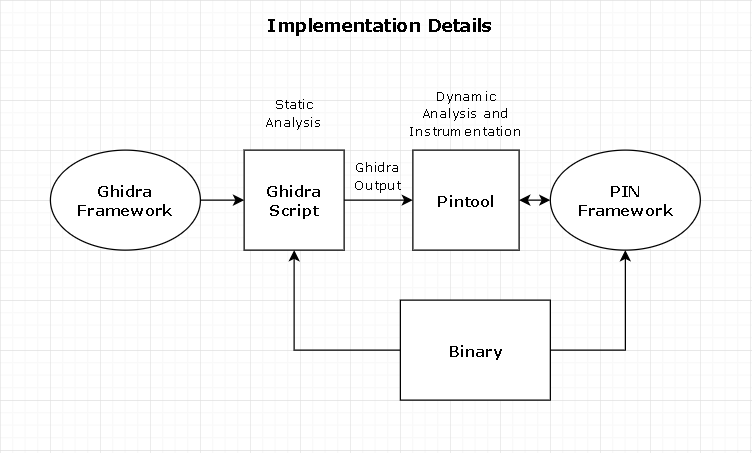
\includegraphics[width=138mm]{images/implementation_details.png}
\caption{Implementation Details\label{fig:fig36}}
\par\end{centering}
\end{figure}